\frame
{
\frametitle{Experiments}
\framesubtitle{Hardware and Software configuration}
\begin{itemize}
    \item CPU: 16 x Intel(R) Xeon(R) CPU E5520  @ 2.27GHz
    \item RAM: 12 GB
    \item Graphic Card: 2 x nVidia Tesla C1060.
    \begin{itemize}
        \item 1 GPU with 240 cores @ 1.3 GHz
        \item Memory: 4GB
    \end{itemize}
    \item OS: Scientific Linux SL release 5.6 (Boron)
    \item Kernel: 2.6.18-238.12.1.el5 x86\_64 GNU/Linux
\end{itemize}
}


\frame
{
\frametitle{Experiments}
\framesubtitle{OpenMP}
\begin{center}
    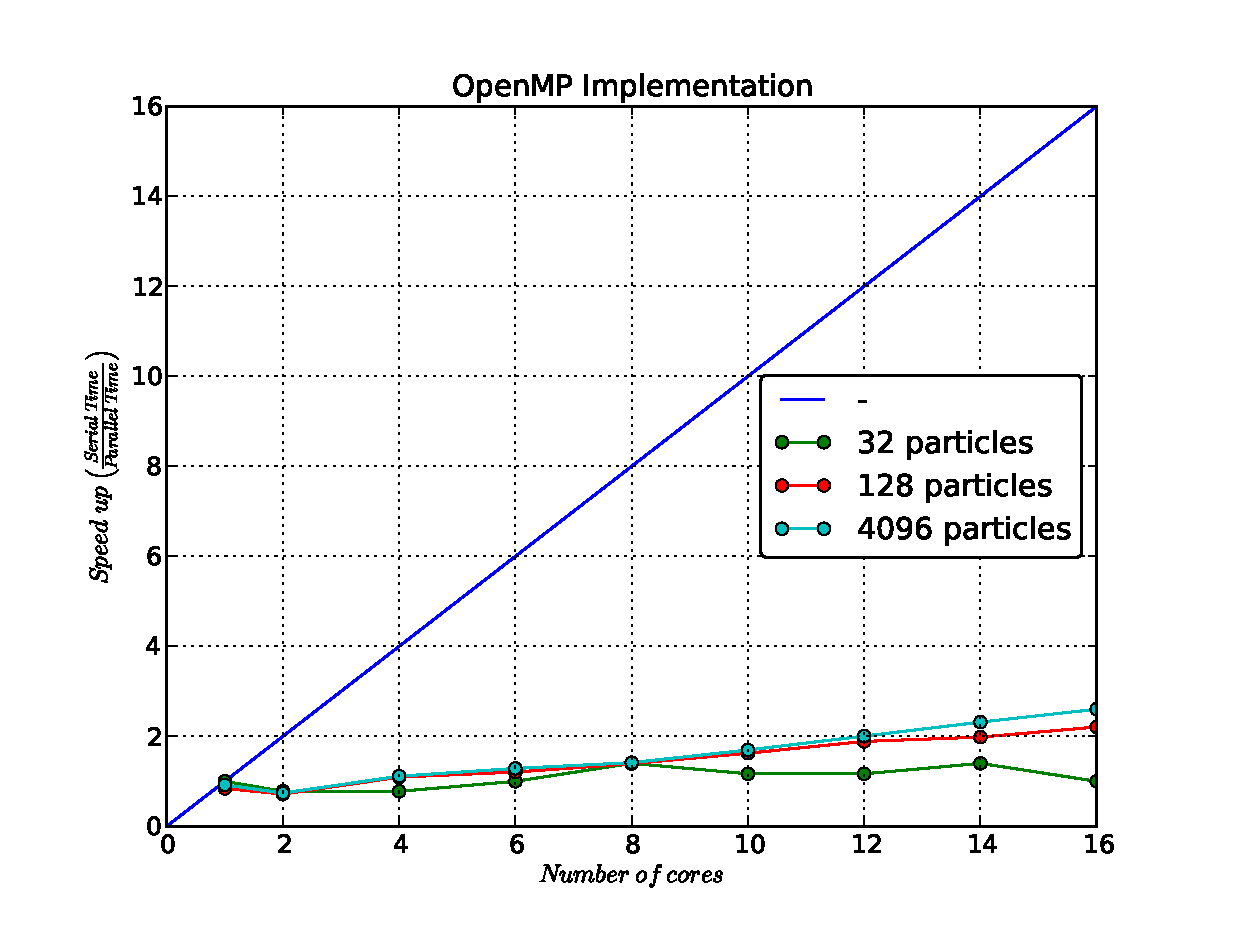
\includegraphics[width=0.8\textwidth]{img/openmp}
\end{center}
}

\frame
{
\frametitle{Experiments}
\framesubtitle{Pthreads}
\begin{center}
    \includegraphics[width=0.8\textwidth]{img/pthreads}
\end{center}
}

\frame
{
\frametitle{Experiments}
\framesubtitle{CUDA}
\begin{center}
    \includegraphics[width=0.8\textwidth]{img/cuda}
\end{center}
}

\frame
{
\frametitle{Experiments}
\framesubtitle{General}
\begin{center}
    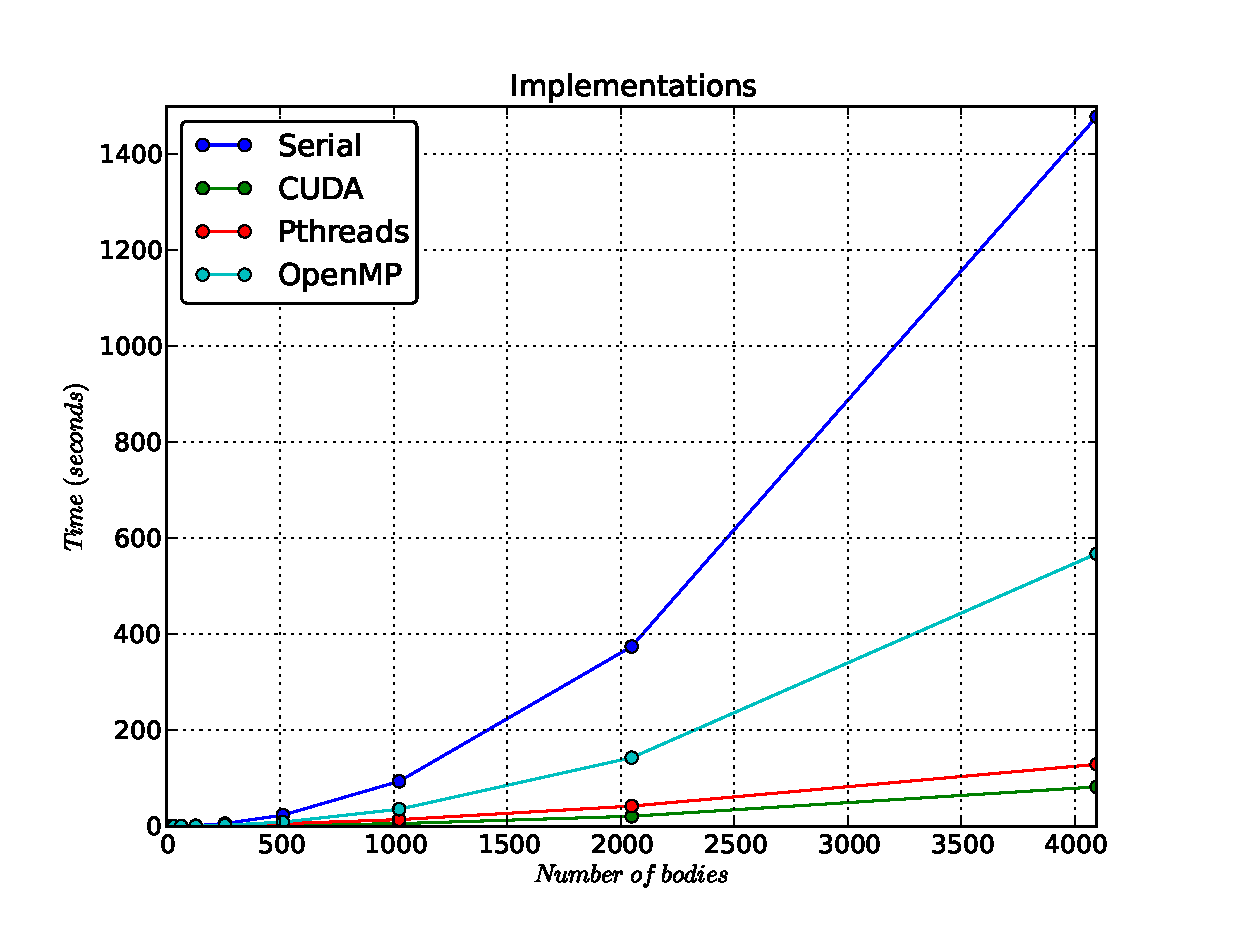
\includegraphics[width=0.8\textwidth]{img/all}
\end{center}
}

\frame
{
\frametitle{Experiments}
\framesubtitle{Acceleration}
\begin{center}
    \begin{tabular}{|c|c|}
        \hline
        \textbf{Implementation} & \textbf{Speed-up} \\\hline
        Serial  & 1x  \\\hline
        OpenMP  & 3x  \\\hline
        Pthread & 11x \\\hline
        CUDA    & 18x \\\hline
    \end{tabular}
\end{center}
}

\frame
{
\frametitle{Experiments}
\framesubtitle{Conclusions}

\begin{itemize}
    \item<1-> Algorithm \red{Granularity} $\rightarrow$ CPU or GPU.
    \item<2-> Benefit/Cost (Money, Programming)
    \item<3-> Application area.
\end{itemize}

}


\begin{frame}[fragile]
\frametitle{Appendix}
\framesubtitle{OpenMP}
\begin{lstlisting}[style=C]
void updateAccelerations(){
    int i,j;
    for (i = 0; i < n; i++) {
        bodies[i].ax = bodies[i].ay = bodies[i].az = 0;
    }
    #pragma omp parallel for private(j)
    for (i = 0; i < n; i++) {
        for(j=0; j<n; j++){
            if(j != i)
                accelerationCalc(i,j);
        }
    }
}
\end{lstlisting}
\end{frame}

\begin{frame}[fragile]
\frametitle{Appendix}
\framesubtitle{Pthreads}
\begin{lstlisting}[style=C]
void updateAccelerations(){
    int i;

    for (i = 0; i < n; i++) {
        bodies[i].ax = bodies[i].ay = bodies[i].az = 0;
    }
    int bound = n/cores;
    for (i = 0; i < cores; i++) {
        threads[i].ini = i * bound;
        threads[i].end = threads[i].ini + bound;
        pthread_create(&threads[i].thread, NULL , accelerationCalc, (void *)&threads[i]);
    }

    for(int j=0 ; j < cores ; ++j){
        pthread_join(threads[j].thread, NULL);
    }

}
\end{lstlisting}
\end{frame}

\begin{frame}[fragile]
\frametitle{Appendix}
\framesubtitle{CUDA}
\begin{lstlisting}[style=C]
__device__ void update_accelerations(particle *d_bodies,int n){

    int i = threadIdx.x + blockDim.x * blockIdx.x;
    int j;

    if (i < n){
        for(j=0; j<n; j++){
            if(j != i)
                accelerationCalc(i,j);
        }
    }
}
\end{lstlisting}
\end{frame}


\begin{frame}[fragile]
\frametitle{Appendix}
\framesubtitle{CUDA}

\begin{lstlisting}[style=C]
  nbody<<< blockNum, threadsPerBlock >>> (d_bodies,ite,dt,n);
  cudaThreadSynchronize();
\end{lstlisting}

\begin{lstlisting}[style=C]
__global__ void nbody(particle *d_bodies,float ite, float dt, int n){

    float t;
    reset_accelerations(d_bodies,n);
    __syncthreads();
    update_accelerations(d_bodies, n);
    __syncthreads();

    for (t = 0.0; t < ite; t += dt){
        update_positions(d_bodies,dt,n);
        __syncthreads();
        reset_accelerations(d_bodies,n);
        __syncthreads();
        update_accelerations(d_bodies,n);
        __syncthreads();
        update_velocities(d_bodies,dt,n);
        __syncthreads();
    }
}
\end{lstlisting}
\end{frame}
